\documentclass[border=0mm]{standalone}

\usepackage{import}
\subimport{../../../}{preamble.tex}

\usepackage{tikz}
\usetikzlibrary{calc}
\usepackage{pgfplots}
\usepgfplotslibrary{fillbetween}

\renewcommand{\t}{-5}

\begin{document}

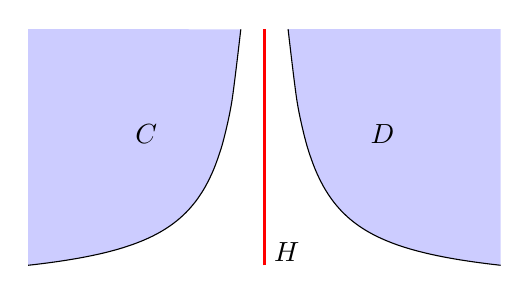
\begin{tikzpicture}
  
  \fill[domain=0.3:3,smooth,variable=\x,fill=blue!20] plot ({\x},{1/\x}) -- (3,1/0.3) -- cycle;
  \draw[domain=0.3:3,smooth,variable=\x,draw=black] plot ({\x},{1/\x}) ;
  \node at (1.5,2) {$D$};

  \fill[domain=-3:-0.3,smooth,variable=\x,fill=blue!20] plot ({\x},{1/-\x}) -- (-3,1/0.3) -- cycle;
  \draw[domain=-3:-0.3,smooth,variable=\x,black] plot ({\x},{1/-\x});
  \node at (-1.5,2) {$C$};

  \draw[red, line width=1pt] (0,1/3)--(0,1/0.3);
  \node[right] at (0,0.5) {$\red{H}$};
  
\end{tikzpicture}

\end{document}

%%% Local Variables:
%%% mode: latex
%%% TeX-master: t
%%% End:
